%% This tex file reads files.lst and generates the pdf from the files listed
%% in there, don't run this directly instead run the Makefile


\documentclass{article}
\usepackage[landscape,twocolumn,nomarginpar,height=7in,width=10in,top=1in,bottom=0.5in,columnsep=0.5in,headsep=.1in]{geometry}
\usepackage[T1]{fontenc}
\usepackage{fancyvrb}
\usepackage{fancyhdr}
\usepackage{listings}
\usepackage{caption}
\usepackage{color}
\usepackage{pdfpages}
\usepackage{tikz}
\usepackage{amsmath}

\pagestyle{fancy}
\lhead[University of Wisconsin - Madison]{University of Wisconsin - Madison}
\rhead[\thepage]{\thepage}
\lfoot[]{}
\cfoot[]{}
\rfoot[]{}

\def\cleanws#1 {#1}
\def\stripslash#1#2\ssend{#2}
\def\makesane[#1]{\expandafter\expandafter\expandafter\stripslash\expandafter\string\csname#1\endcsname\ssend}

\lstloadlanguages{[GNU]C++,Java}
\lstset{
basicstyle=\fontsize{7pt}{8.1pt}\ttfamily,
keywordstyle=\color{blue}\bfseries,
language=[GNU]C++,
columns=fixed,
numbers=left,numberstyle=\tiny,
linewidth=5in,
breaklines=true,
basewidth={0.6em,0.45em},
frame=lines,
}
\renewcommand\listfigurename{Entries}
\begin{document}
\lstlistoflistings
\newread\fstream
\openin\fstream=files.lst
\loop
\def\test{a}
\ifeof\fstream
\def\test{\relax}
\fi
\if a\test
\read\fstream to \fname
\if\fname\par
\relax
\else
\edef\fname{\expandafter\cleanws\fname}
\edef\fname{\makesane[\fname]}
\edef\fname{\noexpand\detokenize{\fname}}
\lstinputlisting[caption={[\noexpand\noexpand\noexpand\detokenize{\fname}]},title={\fname},name=\fname]{\fname}
\fi
\repeat
\newpage

\section{Linear Algebra}

$proj_\mathbf{b}\left(\mathbf{a}\right) = \frac{\mathbf{a} \cdot \mathbf{b}}{\left\|\mathbf{b}\right\|}\frac{\mathbf{b}}{\left\|\mathbf{b}\right\|}$

To solve a non-hoomogenous system, i.e. $A\cdot x = c$, then first solve the homogenous system $A\cdot x = 0$, This gives a subspaces $V$ of solutions, then the affine space of solutions to $A\cdot x = c is V + A^{-1}c$ where $A^{-1}c$ is any solution to $A\cdot x = c$



\section{Trig Identities}
\begin{gather*}
  \sin^2 + \cos^2 = 1\\
  \sin\left(a \pm b\right) = \sin a\cos b \pm \cos a \sin b\\
  \cos\left(a \pm b\right) = \cos a\cos b \mp \sin a \sin b\\
  \tan\left(a \pm b\right) = \frac{\tan a \pm \tan b}{1\mp \tan a \tan b}\\
  \cos\left(nx\right) = 2 \cos x \cos \left(\left(n-1\right)x\right) - \cos\left(\left(n-2\right)x\right)\\
  \sin\left(nx\right) = 2 \cos x \sin \left(\left(n-1\right)x\right) - \sin\left(\left(n-2\right)x\right)
\end{gather*}



\section{Calculus}

\[\begin{array}{|c|c|c|}
\hline
f\left(x\right) & \int f dx & \frac{d}{dx}f\\\hline \hline
\cos x & \sin x & -\sin x\\\hline
\sin x & -\cos x & \cos x\\\hline
\sec x & \ln\left|\sec x + \tan x\right| & \sec x \tan x\\\hline
\csc x & \ln\left|\csc x - \cot x\right| & -\csc x \cot x\\\hline
\tan x& -\ln\left|\cos x\right| & \sec^2 x\\\hline
\cot x & \ln\left|\sin x\right| & -\csc^2 x\\\hline
\sinh x & \cosh x & \cosh x\\\hline
\cosh x & \sinh x & \sinh x\\\hline
\tanh x & \ln \left(\cosh x\right) & 1-\tanh^2 x\\\hline
\arctan x & x \arctan x - \frac{1}{2} \ln \left|1+x^2\right| & \frac{1}{1+x^2}\\\hline
\arcsin x & x \arcsin x + \sqrt{1-x^2}& \frac{1}{\sqrt{1-x^2}}\\\hline
\arccos x & x \arccos x - \sqrt{1-x^2}& \frac{-1}{\sqrt{1-x^2}}\\\hline
\ln x & x\ln x - x & \frac{1}{x}\\\hline
\end{array}
\]


\section{Number theory}

\[\phi\left(p_1^{e_1}\cdots p_n^{e_n}\right)=\prod_{i=1}^{n}p_i^{e_i-1}\left(p_i-1\right)\]


Primes under 1000:\\
2, 3, 5, 7, 11, 13, 17, 19, 23, 29, 31, 37, 41, 43, 47, 53, 59, 61, 67, 71, 73, 79, 83, 89, 97, 101, 103, 107, 109, 113, 127, 131, 137, 139, 149, 151, 157, 163, 167, 173, 179, 181, 191, 193, 197, 199, 211, 223, 227, 229, 233, 239, 241, 251, 257, 263, 269, 271, 277, 281, 283, 293, 307, 311, 313, 317, 331, 337, 347, 349, 353, 359, 367, 373, 379, 383, 389, 397, 401, 409, 419, 421, 431, 433, 439, 443, 449, 457, 461, 463, 467, 479, 487, 491, 499, 503, 509, 521, 523, 541, 547, 557, 563, 569, 571, 577, 587, 593, 599, 601, 607, 613, 617, 619, 631, 641, 643, 647, 653, 659, 661, 673, 677, 683, 691, 701, 709, 719, 727, 733, 739, 743, 751, 757, 761, 769, 773, 787, 797, 809, 811, 821, 823, 827, 829, 839, 853, 857, 859, 863, 877, 881, 883, 887, 907, 911, 919, 929, 937, 941, 947, 953, 967, 971, 977, 983, 991, 997


\section{Geometry}




%Right Triangles
%\tikz {
%\draw (0,0) -- node[anchor=east] {b} (0,3) node[anchor=north west] {$\phi$} -- %node[anchor=south west] {c} (5,0) node[anchor=east] {$\theta$} -- node[anchor=north] {a} (0,0);
%\draw (0,0.25) -- (0.25,0.25) -- (0.25,0);
%}

%arbitrary triangles

%\begin{tikzpicture}
%  \draw (0,0) circle (3);
%  \node (A) at (canvas polar cs:angle=10,radius=3cm) {};
%  \node (B) at (canvas polar cs:angle=130,radius=3cm) {};
%  \node (C) at (canvas polar cs:angle=220,radius=3cm) {};
%  \draw (A.center) -- node (AB) {} (B.center) -- node (BC) {} (C.center) -- node (AC) {} (A.center);
%  \draw [name path=A-median] (A.center) -- (BC.center);
%  \draw [name path=B-median] (B.center) -- (AC.center);
%  \draw (C.center) -- (AB.center);
%  \draw [name intersections={of=A-median and B-median, by={centroid}}] node at (centroid) {centroid};
%  \draw node (circcenter) at (0,0) {circumcenter};
%  \draw (0,0) -- (AB.center);
%  \draw (0,0) -- (BC.center);
%  \draw (0,0) -- (AC.center);
%  
%\end{tikzpicture}

\subsection{Triangles}

For Barycentric Coordinates in this table, they are NOT normalized, so the location of the point $n : m : p$ is $(n*A+m*B+p*C)/(n+m+p)$. Also a=length of side opposite of the vertex A, and A = angle at vertex A


\begin{tabular}{|c|c|c|}
\hline 
\multicolumn{3}{|c|}{Triangle Centers}\\\hline
Use what & to find & Barycentric Coordinates \\ \hline\hline
Medians & Centroid & $1:1:1$\\\hline
Perpendicular Bisectors & Circumcenter & $ \sin 2A : \sin 2B : \sin 2C $\\\hline
Angle Bisectors & Incenter& $a : b : c$\\\hline
Altitudes & Orthocenter & $\tan A : \tan B : \tan C$\\\hline
\end{tabular}



%TODO circle

%\tikz{
%\draw (0,0) circle (2);
%\draw (0,0) -- (canvas polar cs:angle=0,radius=2cm);
%\draw (0,0) -- (canvas polar cs:angle=30,radius=2cm);
%\draw (canvas polar cs:angle=30,radius=2cm) |- (0,0);
%}

%\tikz{
%\draw (0,0) circle (2);
%\draw (0,0) node[anchor=south] {$2\theta$} -- (canvas polar cs:angle=60,radius=2cm);
%\draw (0,0) -- (canvas polar cs:angle=120,radius=2cm);
%\draw (canvas polar cs:angle=-90,radius=2cm) node[anchor=south] {$\theta$} -- (canvas polar cs:angle=60,radius=2cm);
%\draw (canvas polar cs:angle=-90,radius=2cm) -- (canvas polar cs:angle=120,radius=2cm);
%}

Thm (Power of a Point) For any circle $C$ and any point $P$, if $l$ is a line through $P$ intersecting $C$ at points $A$,$B$ (note, we count multipliciyt) then the value $PA \cdot PB$ is invarient, this value (up to sign) is called the power of the point. Additionally, this value is (up to sign) equal to $s^2-r^2$ where $s$ is the distance of $P$ to the center of $C$ and $r$ is the radius of $C$.


%volumes and areas

\subsection{Polygons}

Given a polygon defined by points $(x_i,y_i)$ (in order), then the area of that polygon is
\[1/2\sum_{i=1}^{n}x_iy_{i+1} - x_{i+1} y_i\]
where $x_{n+1} = x_{1}$ and $y_{n+1} = y_1$


Similarly, a centroid is
\begin{align*}
  C_x &= \frac{1}{6A} \sum_{i=1}^n (x_i + x_{i+1} )( x_i y_{i+1} - x_{i+1} y_i )\\
  C_y &= \frac{1}{6A} \sum_{i=1}^n (y_i + y_{i+1})( x_i(i)y_{i+1} - x_{i+1}y_i )
\end{align*}

Pick's formula

Area of a polygon with integer verticies.
\[A= i + \frac{b}{2} - 1\]
Where $i = \textrm{\# of inteior points}$ and $b = \textrm{\# of boundary points}$

\subsection{Higher Dimensions}

\noindent
\begin{tabular}{|c|c|}
  \hline
  \multicolumn{2}{|c|}{Volumes}\\\hline
  Cone & $\frac{1}{3}B\cdot h$\\\hline
  Sphere & $\frac{4}{3}\pi r^2$\\\hline
\end{tabular}

\noindent
\begin{tabular}{|c|c|}
    \hline
    \multicolumn{2}{|c|}{Surface Area}\\\hline
    Sphere & $4 \pi r^2$\\\hline
    Right Circular Cone & $\pi\cdot r^2+\pi r \cdot \sqrt{r^2+h^2}$\\\hline
\end{tabular}

For polytope volume calculation, reduce to a cone by this algorithm:

First choose any point in the interior of the polytope (including boundary points) then from this point, make a cone to every face of the polytope. Finally, sum the volumes of these cones.



\onecolumn
%{\center 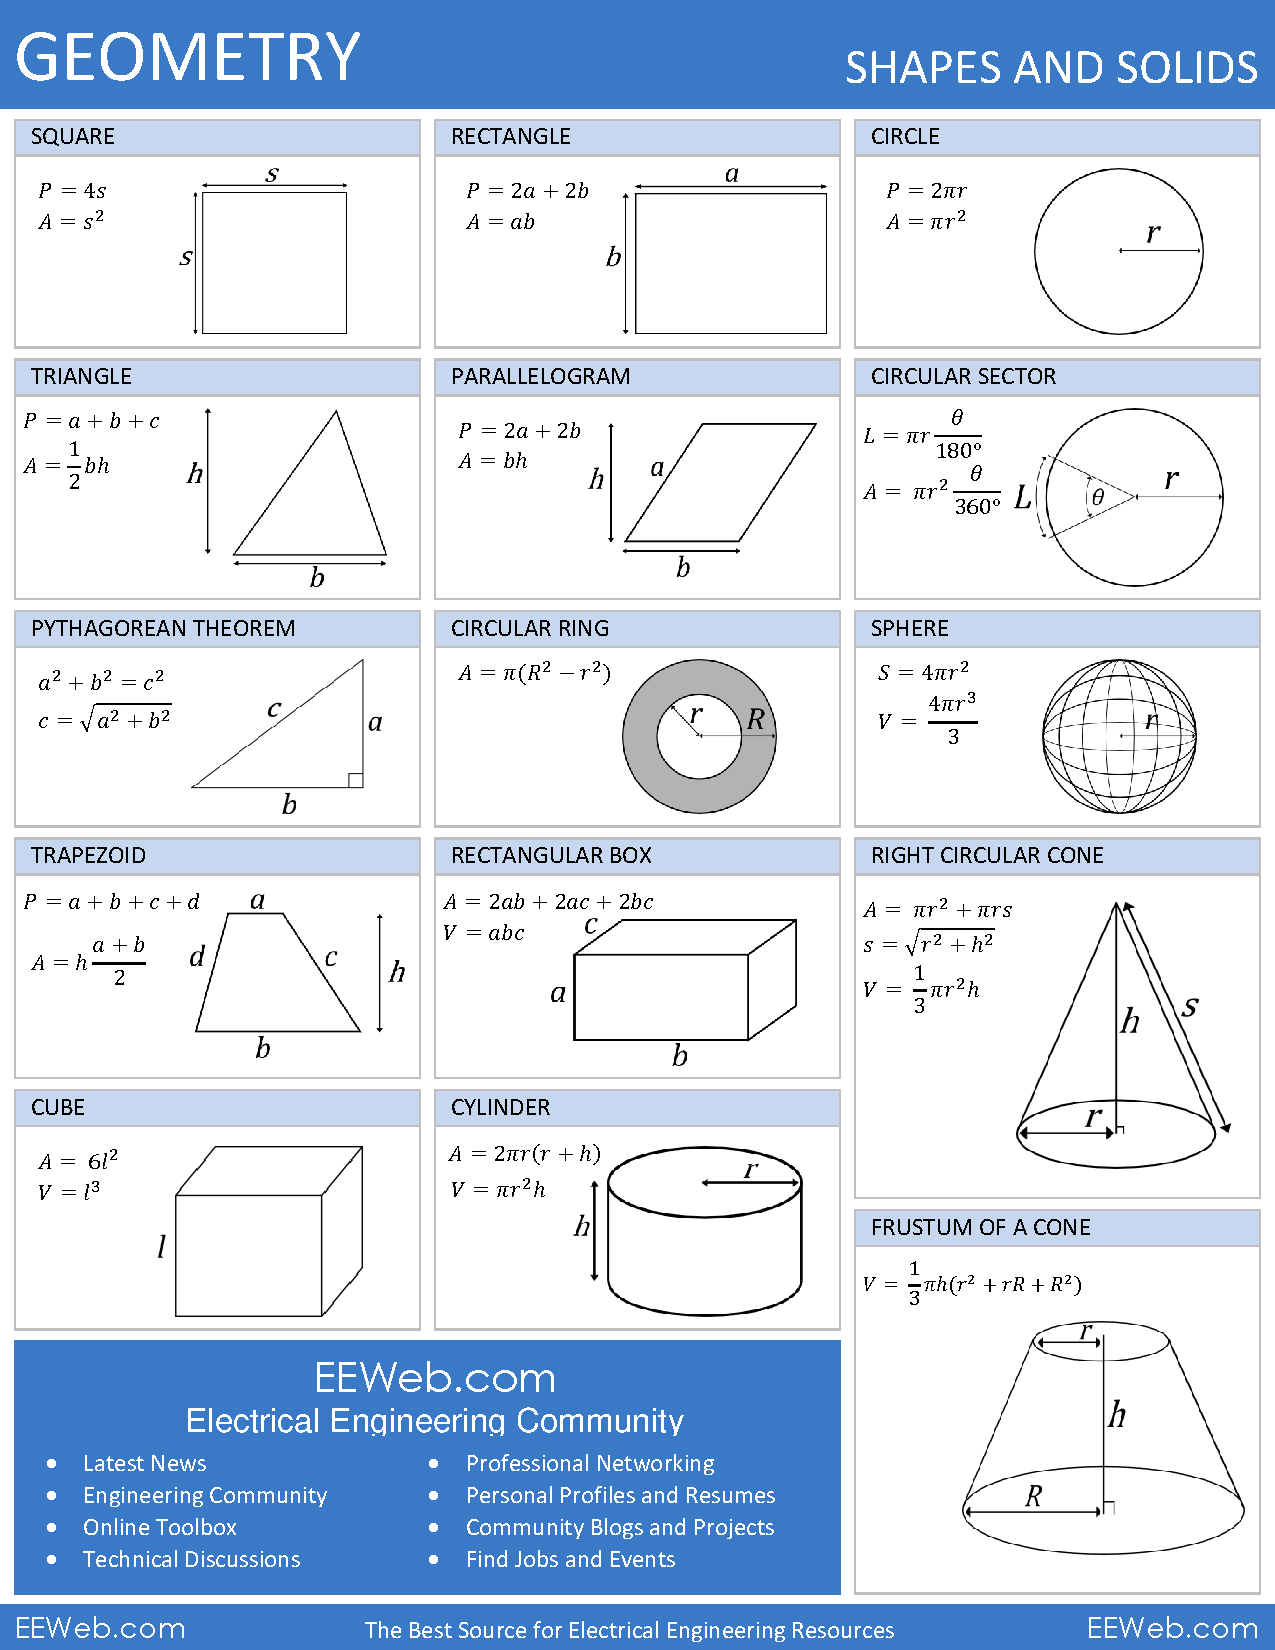
\includegraphics[angle=270,scale=.82]{geom_cheatsheet.pdf}}


\end{document}
